\documentclass[a4paper, 12pt, openright, oneside]{article}


\usepackage{graphicx}			% usar gráficos
\usepackage{multicol,lipsum}	%
\usepackage[utf8]{inputenc}		% Codificacao do documento (conversão automática dos acentos)
\usepackage{indentfirst}		% Indenta o primeiro parágrafo de cada seção.
\usepackage{color}				% Controle das cores
\usepackage{graphicx}			% Inclusão de gráficos
\usepackage{microtype} 			% para melhorias de justificação
\usepackage{natbib} 			% citar
\usepackage{float}				% números em ponto flutuante
\usepackage[brazil]{babel}		% língua brasileira
\usepackage{setspace}			% espaçamento entre linhas
\usepackage[brazilian,hyperpageref]{backref}	 % Paginas com as citações na bibl

\usepackage{amsmath, amsfonts, amssymb}
\usepackage[top=3cm, bottom=2cm, left=3cm, right=2cm]{geometry}

\parskip15pt					% distância entre parágrafos fixa
\parindent30pt					%identação fixa
\everymath{\displaystyle} %farc tamanho ideal

% ---
% Pacotes de citações
% ---
\usepackage[brazilian,hyperpageref]{backref}	 % Paginas com as citações na bibl
\usepackage[alf]{abntex2cite}	% Citações padrão ABNT

%----------------------
% Pacotes para a linha de código
%----------------------
\usepackage{xcolor}
% Definindo novas cores
\definecolor{verde}{rgb}{0,0.5,0}
% Configurando layout para mostrar codigos C++
\usepackage{listings}
\lstset{
  language=Fortran,
  basicstyle=\ttfamily\small,
  keywordstyle=\color{blue},
  stringstyle=\color{verde},
  commentstyle=\color{red},
  extendedchars=true,
  showspaces=false,
  showstringspaces=false,
  numbers=left,
  numberstyle=\tiny,
  breaklines=true,
  backgroundcolor=\color{green!10},
  breakautoindent=true,
  captionpos=b,
  xleftmargin=0pt,
}
\pagestyle{empty}
%----------------------
%----------------------

% --- 
% CONFIGURAÇÕES DE PACOTES
% --- 

% ---
% Configurações do pacote backref
% Usado sem a opção hyperpageref de backref
\renewcommand{\backrefpagesname}{Citado na(s) página(s):~}
% Texto padrão antes do número das páginas
\renewcommand{\backref}{}
% Define os textos da citação
\renewcommand*{\backrefalt}[4]{
	\ifcase #1 %
		Nenhuma citação no texto.%
	\or
		Citado na página #2.%
	\else
		Citado #1 vezes nas páginas #2.%
	\fi}%
% ---

\begin{document}
%\maketitle
\onehalfspacing
\begin{titlepage}
	\begin{center}
	
	\begin{figure}[!ht]
	\centering
	
\includegraphics[width=2cm]{./ufrn.jpg}
	\end{figure}
		Universidade Federal do Rio Grande do Norte\\
		Centro de Tecnologia\\
		Departamento de Engenharia da Computação e Automação\\
		DCA0304 -- Métodos Computacionais em Engenharia\\
		\vspace{15pt}
        \vspace{95pt}
        \textbf{\large{Comparação entre Julia e outras linguagens de programação na eficiência de execução do método de Newton-Raphson para solução de sistema de equações não-lineares}}\\
		\vspace{3,5cm}
	\end{center}
	
	\begin{flushright}
			\item André Rodrigues Bezerra Madruga \\
			Bruno Matias de Sousa \\
			José Ricardo Bezerra de Araújo \\
			Levy Gabriel da Silva Galvão \\
 	\end{flushright}
	\vspace{1cm}
	
	\begin{center}
		\vspace{\fill}
		Novembro\\2018
	\end{center}
\end{titlepage}
%%%%%%%%%%%%%%%%%%%%%%%%%%%%%%%%%%%%%%%%%%%%%%%%%%%%%%%%%%%

% % % % % % % % %FOLHA DE ROSTO % % % % % % % % % %



\begin{titlepage}
	\begin{center}
	
	\begin{figure}[!ht]
	\centering
	
\includegraphics[width=2cm]{./ufrn.jpg}
	\end{figure}

		Universidade Federal do Rio Grande do Norte\\
		Centro de Tecnologia\\
		Departamento de Engenharia da Computação e Automação\\
		DCA0304 -- Métodos Computacionais em Engenharia\\
\vspace{15pt}
        
        \vspace{85pt}
        
		\textbf{\large{Comparação entre Julia e outras linguagens de programação na eficiência de execução do método de Newton-Raphson para solução de sistema de equações não-lineares}}\\
	%	\large{Modelo\\
     %   		Validação do modelo clássico}
			
	\end{center}
\vspace{1,5cm}
	
	\begin{flushright}

   \begin{list}{}{
      \setlength{\leftmargin}{4.5cm}
      \setlength{\rightmargin}{0cm}
      \setlength{\labelwidth}{0pt}
      \setlength{\labelsep}{\leftmargin}}

      \item Relatório técnico referente à execução prática dos métodos numéricos para a solução de sistemas de equações não-lineares realizado na disciplina de Métodos Computacionais em Engenharia, como requisito parcial para avaliação da terceira unidade da discplina antes mencionada.

      \begin{list}{}{
      \setlength{\leftmargin}{0cm}
      \setlength{\rightmargin}{0cm}
      \setlength{\labelwidth}{0pt}
      \setlength{\labelsep}{\leftmargin}}


            \item Orientador: Profº. Drº. Paulo Sergio da Motta Pires

      \end{list}
   \end{list}
\end{flushright}
\vspace{1cm}
\begin{center}
		\vspace{\fill}
		 Novembro\\2018
			\end{center}
\end{titlepage}
\newpage
% % % % % % % % % % % % % % % % % % % % % % % % % %
\newpage
\tableofcontents
\thispagestyle{empty}

\newpage
\pagenumbering{arabic}
% % % % % % % % % % % % % % % % % % % % % % % % % % %
\section*{Resumo}

Lorem ipsum dolor sit amet, consectetur adipiscing elit. Quisque et gravida mauris. Phasellus at ipsum in nisl iaculis consequat. Fusce vulputate nisl ipsum, quis egestas justo accumsan et. Morbi consequat tellus a eros eleifend congue. Aenean laoreet mattis nunc, at iaculis orci imperdiet in. Donec a diam in sem auctor fringilla. Aenean euismod odio vel arcu pretium, in vehicula urna ultricies. 

 \noindent
 \textbf{Palavras-chaves}: métodos. computacionais. engenharia.
\newpage

% ----------------------------------------------------------
% ELEMENTOS TEXTUAIS
% ----------------------------------------------------------

% ----------------------------------------------------------
% Introdução 
% ----------------------------------------------------------

\section{Introdução}

\pagestyle{myheadings}
\markright{ }

Muitos problemas da ciência da computação e de outras ciências podem serem abstraídos por meio de fórmulas e equações provenientes de uma linguagem matemática. Algumas dessas equações podem ser solucionadas de forma analítica utilizando a conceituação da literatura da área. Porém muitos outros problemas não possuem solução fechada por um método analítico, assim sendo necessário recorrer aos métodos iterativos, na maioria dos casos.

Ao longo dos anos os métodos iterativos solucionam problemas em diversas áreas, tais como: economia, engenharia, física, biologia, etc. Sua aplicação se baseia na aproximações para a solução do problema que melhoram em precisão de acordo com que aumentam o número de iterações. A extensa literatura na área de métodos iterativos só fortalece a importância de estudar a área.

A natureza repetitiva dos métodos iterativos sugere a sua execuação em recursos computacionais. Assim, a atividade "manufaturada" de realizar os cálculos é transferida para um computador, capaz de executá-las mais rapidamente.

Dessa forma, surgiu com o tempo uma tendência cada vez maior -- de acordo com que a tecnologia se desenvolvia -- de aliar a solução de problemas matemáticos aos métodos computacionais. Principalmente aqueles cuja solução analítica é difícil ou impossível. Um exemplo são os problemas de sistemas de equações não lineares que serão abordados no presente trabalho.

Para a obtenção das soluções desejadas foram utilizadas as linguagens de programação para realizar a comunicação entra a linguagem humana e matemática e a linguagem binária de máquina. Existem diversas linguagens com os mais diversos propósitos. Umas aplicadas ao gerenciamento de bancos de dados e outras com recursos dedicados aos métodos numéricos. 

Com a pluralidade de escolhas, basta ao profissional escolher aquela linguagem que mais se adequa às suas necessidades. O mais procurado nos dias atuais na solução de problemas por métodos numéricos é a linguagem que seja mais rápida, que utilize menos recurso computacional e ofereça a resposta mais precisa. 

Uma linguagem tida como forte candidata à preferida no cálculo numérico é a Julia. Uma linguagem bastante recente, cujo desenvolvimento começou em 2009 e teve a primeira versão de código aberto lançada em 2012.


\newpage

\section{Desenvolvimento}

Lorem ipsum dolor sit amet, consectetur adipiscing elit. Quisque et gravida mauris. Phasellus at ipsum in nisl iaculis consequat. Fusce vulputate nisl ipsum, quis egestas justo accumsan et. Morbi consequat tellus a eros eleifend congue. Aenean laoreet mattis nunc, at iaculis orci imperdiet in. Donec a diam in sem auctor fringilla. Aenean euismod odio vel arcu pretium, in vehicula urna ultricies.

Vivamus ut pharetra diam. Aliquam metus sem, tristique ac dignissim eu, pretium id velit. Donec id tincidunt odio. Fusce vehicula ac est quis convallis. Nullam sollicitudin euismod dolor, eget blandit turpis hendrerit at. In bibendum suscipit odio, at consequat erat laoreet id. Donec in tellus at nulla gravida egestas. Suspendisse non elementum leo. Nam viverra sapien sed velit tempor scelerisque. Nunc accumsan odio eget mi vehicula, vel interdum libero gravida. Pellentesque vitae molestie diam, quis vestibulum libero. Aenean finibus sapien diam, ac sagittis magna placerat nec. Ut maximus eros felis, vel egestas diam convallis sit amet. Integer interdum elementum turpis, sit amet luctus nisi scelerisque at. Donec eleifend arcu dictum metus ullamcorper tempor. Aenean placerat, arcu id suscipit vehicula, velit ipsum viverra lorem, et pretium velit tellus quis libero.

\subsection{Newton-Raphson para sistema de equações não-lineares}
Nunc accumsan odio eget mi vehicula, vel interdum libero gravida. Pellentesque vitae molestie diam, quis vestibulum libero. Aenean finibus sapien diam, ac sagittis magna placerat nec. Ut maximus eros felis, vel egestas diam convallis sit amet. Integer interdum elementum turpis, sit amet luctus nisi scelerisque at. Donec eleifend arcu dictum metus ullamcorper tempor. Aenean placerat, arcu id suscipit vehicula, velit ipsum viverra lorem, et pretium velit tellus quis libero.

\subsection{Sistema de equações propostos}

Os sistemas considerados para a solução são dois. Um contendo três varáveis e outro com duas. Aquele que possui três variáveis será chamado de sistema 1 (sis\_1). O outro será o sistema 2 (sis\_2).

A seguir estão apresentados os sistemas. Vale salientar que o sistema 2 possui resposta dada em radiano, uma vez que as variáveis $x_1$ e $x_2$ compõem o argumento de uma função senoidal.


\begin{itemize}
\item $ x_2 + x_3 - e^{-x_1} = 0$
\item $ x_1 + x_3 - e^{-x_3} = 0$
\item $ x_1 + x_2 - e^{-x_3} = 0$
\end{itemize}
\bigskip 
\begin{itemize}
\item $ \frac{1}{2}sen(x_1x_2) - \frac{x_2}{4\pi} - \frac{x_1}{2}  = 0$
\item $ (1-\frac{1}{4\pi})(e^{2x_1}-e) - \frac{ex_2}{\pi} - 2ex_1 = 0$
\end{itemize}


\subsection{Fluxograma do algoritmo}
Na execuação dos códigos o algoritmo base se permaneceu o mesmo, apesar de ele ser aplicado em três linguagens diferentes (Fortran 95, Julia e Python).

O algoritmo será descrito a seguir por meio de fluxogramas. Contudo, os códigos completos referentes às linguagens Fortran 95, Julia e Python se encontram no apêndice. 

O código principal será executado na \textit{main} cujo algoritmo se baseia em passar alguns parâmetros para que a função new\_rap possa executar o algoritmo de Newton--Raphson para a resolução do sistema de equações não-lineares retornando um vetor com as soluções.

Os parâmetros que são passados é um vetor $x0$ contendo os chutes iniciais. Para critério de parada é utilziada uma tolerância que irá indicar a precisão de execução (geralmente um erro na ordem de $10^{-12}$) e o número de iterações.

\begin{figure}[!htb]
\centering
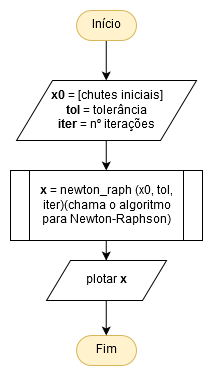
\includegraphics[scale=0.6]{Imagens/diag_main.png}
\caption{Fluxograma da main, função principal para executar o programa. Fonte: própria.}
\label{galvanometro}
\end{figure}

O próximo fluxograma indicará a execução da função newton\_raph() para a execução do algoritmo de Newton--Raphson. Ele irá utilizar os chutes iniciais e irá armazenar os valores da função em um vetor através de uma função f() e armazenar os valores do jacobiano pela função jac() para aquele dado chute. Em seguida irá resolver o sistema linear dado pela matriz jacobiana obtida com o vetor de resposta dado pelo oposto dos valores dados pelo vetor de valores da função. Para solução desse sistema será utilizado a fatoração LU por meio de uma função LU().

Após obter a solução do sistema linear, a solução para o sistema de equações não lineares será a soma da solução linear com o chute anterior. Logo após isso, os critérios de parada serão verificados e se caso o valor máximo absoluto dos valores da função para aquele chute forem maior que a tolerância ou o número de iterações ultrapassar a quantidade estipulada, o algoritmo irá parar e retorna a solução para o sistema não-linear. Porém caso esses critérios não forem verdadeiros o algoritmo se repetirá com o vetor de chutes inicias sendo substituído pela atual resposta do sistema não-linear.

\begin{figure}[!htb]
\centering
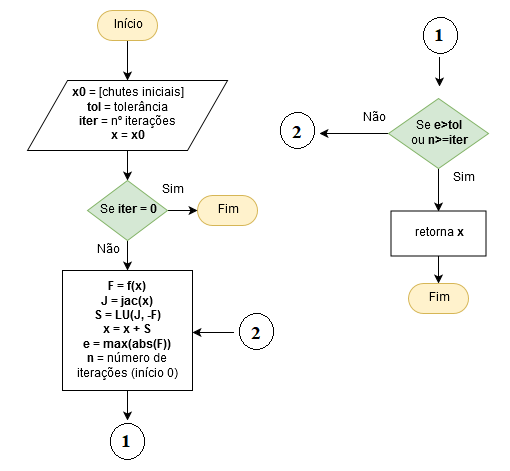
\includegraphics[scale=0.7]{Imagens/diag_new1.png}
\caption{Fluxograma da função newton\_raph() que calcula um vetor de soluções para um sistema de equações não-linear. Fonte: própria.}
\label{galvanometro}
\end{figure}

Os fluxogramas restantes descrevem, respectivamente o funcionamento da função f() que recebe as coordenadas do ponto e retorna um vetor com os valores da função. A função jac() retorna a matriz jacobiana a partir das coordenadas do ponto por meio de um cálculo numérico de derivadas. Por fim, a função LU() realiza a fatoração LU e resolve o sistema linear a partir de uma dada matriz e um vetor resposta. As figuras referentes a esses três últimos fluoxgramas se encotram no apêndice de fluxogramas.

\newpage

\section{Resultados}

Para a análise dos resultados fora utilizado o seguinte hardware e software:

\begin{itemize}
 \item Sistema Operacional Microsoft Windows 10 Home Single Language;
 
 \item Processador Intel® Core(TM) i5-8250U Quadri Core 2.5 GHz com Turbo Max até 3.4 GHz;
 
 \item Placa de vídeo dedicada Geforce MX150 2 GBIntel® HD Graphics 620;
 
 \item Memória RAM 8GB DDR4 2133 MHz;
 
 \item Disco rígido (HD) 1 TB 5400 RPM.
\end{itemize}

Como IDE para a linguagem Fortran foi utilizado o CodeBlocks com o compilador gcc 5.1.0. Para a linguagem Julia com a versão 1.0.1 foi usada a IDE Juno. Finalmente, para Python foi utilizada a versão 3.7 com a IDE PyCharm.
  
\subsection{Raízes}

O primeiro sistema (sis\_1) possui apenas duas soluções de acordo com a análise do gráfico em três dimensões da intersecção dos planos gerados por cada equação. Porém o segundo sistema (sis\_2) possui infinitas soluções devido a natureza periódica da intereseção entre as duas curvas em duas dimensões. 

A tabela a seguir refere-se às soluções encontradas para cada sistema a partir de um dado chute inicial.

\begin{table}[htbp]
  \centering
  \caption{Soluções encontradas para um dado chute inicial (o número após o prefixo sis\_ se refere a qual o sistema a solução se refere e o número após o sufixo \_sol se refere ao número da solução). Fonte: própria.}
    \begin{tabular}{|c|c|c|}
\multicolumn{1}{c|}{} & \textbf{Solução} & \textbf{Chute inicial} \\

    sis\_1\_sol1 & [0.35173371, 0.35173371, 0.35173371]  & [0.5, 0.5, 0.5] \\

    sis\_1\_sol2 & [-0.83202504,  1.14898375,  1.14898375]  & [0, 1, 2] \\
 
    sis\_2\_sol1 & [0.11116545 -2.26144905]  & [0.5, -2] \\

    sis\_2\_sol2 & [-0.52596071,  0.78465031] & [0, 0] \\

    sis\_2\_soln & [-4.28925635, 24.05879992]  & [0.25, 0.25] \\

    \end{tabular}%
  \label{tab:addlabel}%
\end{table}%

Para o segundo sistema foram analisadas apenas três das infinitas soluções, enquanto que para o primeiro sistema foram encontradas as duas únicas soluções. 

De acordo com cada chute inicial o algoritmo convergia mais facilmente para uma dada solução. No segundo sistema para outros valores de chute inicial podem ser encontradas mais soluções, enquanto que no primeiro o algoritmo só converge para as duas soluções apresentadas.

Em complemento às raízes encontradas, os gráficos das curvas podem ser plotados para uma melhor compreensão da solução encontrada. No primeiro sistema cujo gráfico das curvas é dado em três dimensões (3D) a visualização se torna possível, porém de difícil compreensão. Já o segundo sistema envolve apenas duas variáveis, permitindo a visualização de um gráfico em duas dimensões (2D).

O gráfico do segundo sistema se encontra na figura abaixo obtida pela biblioteca \textit{matplotlib} do Python.

\begin{figure}[!htb]
\centering
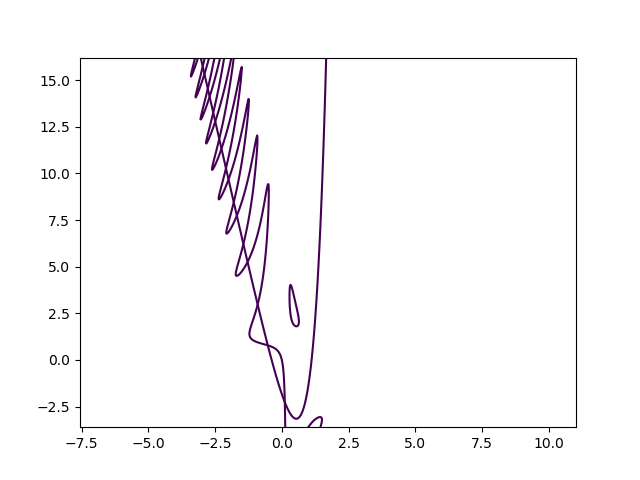
\includegraphics[scale=0.7]{Imagens/2d.png}
\caption{Gráfico das curvas do segundo sistema obtido pela linguagem Python. Fonte: própria.}
\label{galvanometro}
\end{figure}

Como ambas as equações do sistema estão igualadas a zero, indica que a solução está em um ponto comum a elas (onde elas se cruzam), como pode ser observado no gráfico da figura acima. 



\subsection{Eficiência na execução}

Para a comparação do tempo de execução do algoritmo de Newton--Raphson por cada linguagem, foram estabelecidos alguns chutes iniciais em cada linguagem e logo após medidos os tempos.

O gráfico da figura abaixo mostra os valores de tempo absoluto em segundos para cada linguagem, sistema e solução. Lembrando que o rótulo utilizado para se referenciar a cada sistema e solução segue a mesma regra da tabela na subseção anterior ("raízes").

\begin{figure}[!htb]
\centering
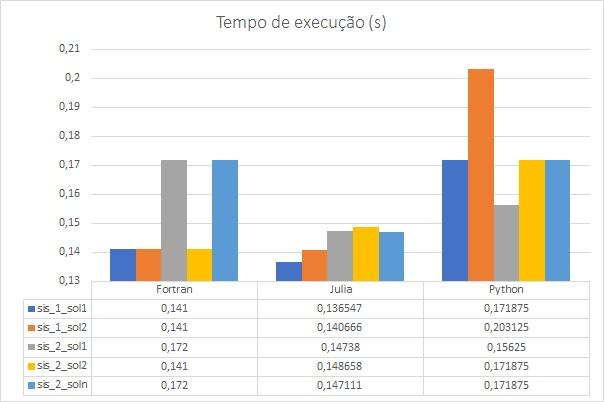
\includegraphics[scale=0.7]{Imagens/graf.jpg}
\caption{Gráfico com os dados de tempo absoluto de execução. Fonte: própria.}
\label{galvanometro}
\end{figure}

Devido a difícil observação e compreensão dos dados no gráfico anterior, fora criada a tabela abaixo para elencar os valores de tempo de execução de cada linguagem normalizada em referência à linguagem Julia. 

\begin{table}[htbp]
  \centering
  \caption{Comparação entre o tempo de execução do código fonte de cada linguagem, solução e chute inicial normalizados com o tempo de Julia.}
    \begin{tabular}{|c|c|c|c|c|}
   \multicolumn{1}{r|}{} & \textbf{Fortran} & \textbf{Julia } & \textbf{Python} & \textbf{Chute inicial} \\
    \multicolumn{1}{r|}{} & \textit{gcc 5.1.0} & \textit{1.0.1} & \textit{3.7} &  \\
    sis\_1\_sol1 & 1.032   & 1       & 1.258   & [0.5, 0.5, 0.5] \\

    sis\_1\_sol2 & 1.002   & 1       & 1.444   & [0, 1, 2] \\

    sis\_2\_sol1 & 1.167   & 1       & 1.060   & [0.5, -2] \\

    sis\_2\_sol2 & 0.948   & 1       & 1.156   & [0, 0] \\

    sis\_2\_soln & 1.169   & 1       & 1.175   & [0.25, 0.25] \\

    \end{tabular}%
  \label{tab:addlabel}%
\end{table}%

Assim, com essa tabela a comparação do tempo de execução entre as linguagens fica mais evidente.

\newpage

\section{Conclusões}

A linguagem de programação JULIA apresentou um desempenho considerável em relação ao tempo de execução do programa apresentado para resolução do sistema não lineares, percebemos que Julia foi de longe, a forma mais rápida de achar as soluções do primeiro sistema, e que no geral, o segundo sistema Julia leva vantagem sobre o Python 3. Na solução dos sistemas não lineares utilizando o método de Newton-Raphson percebemos que as três linguagens analisadas, foram de forma eficientemente aplicadas, retornando assim as soluções esperadas, com várias casas decimais, e com erro na ordem de -12 (menos doze). 

De acordo com o trabalho apresentado, a linguagem de programação Julia, devido sua simplicidade de sintaxe e resultados nos testes, apresenta potencial significativo como alternativa as outras linguagens como: Python, Fortran, MATLAB etc. Percebemos também que por se tratar de uma linguagem nova, é uma alternativa de altíssimo peso na computação numérica, destacando por ter um código-fonte livre e por ser uma linguagem Open Source. 

Por fim, analisando como um todo a linguagem notamos que Julia é uma grande linguagem para o futuro, tendo em vista que Softwares como MATLAB se tornam uma maneira inviável para estudantes e pesquisadores, pois o preço é proibitivo para esse público, com isso, estudo que como esses contribuem ainda mais a crescer a comunidade da Julia, para que todos possam conhecer e usufruir dela.


\newpage



% Referências bibliográficas

\nocite{associaccao1989nbr}
\nocite{marconi2003fundamentos}
\bibliographystyle{abbrv}
\bibliography{refs}

%\begin{figure}[!htb]
%\centering
%\includegraphics[height=6cm]{Photos/galvanometro.jpg}
%\caption{Na esquerda, um galvanômetro normalmente usado em circuitos, no centro, um galvanômetro com a estrutura iterna à amostra com fins didáticos e na direita as suas escalas. Fonte: própria.}
%\label{galvanometro}
%\end{figure}

\newpage



\section{Apêndice}
\subsection{Fluxogramas restantes}
\begin{figure}[!htb]
\centering
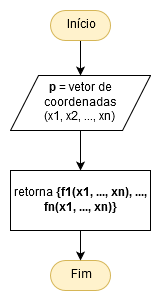
\includegraphics[scale=0.7]{Imagens/diag_func.png}
\caption{Fluxograma da função f() que calcula um vetor de valores do sistema de equação para um dado ponto. Fonte: própria.}
\label{galvanometro}
\end{figure}

\begin{figure}[!htb]
\centering
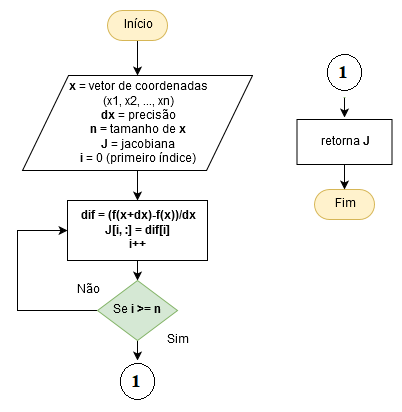
\includegraphics[scale=0.7]{Imagens/diag_jac1.png}
\caption{Fluxograma da função jac() que calcula a matriz jacobiana para um dado ponto. Fonte: própria.}
\label{galvanometro}
\end{figure}

\begin{figure}[!htb]
\centering
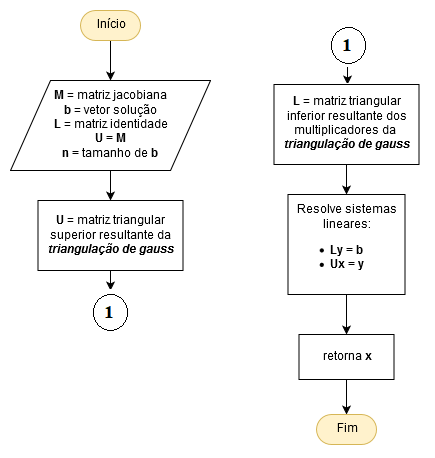
\includegraphics[scale=0.7]{Imagens/diag_LU1.png}
\caption{Fluxograma da função LU() que soluciona um sistema linear por fatoração LU. Fonte: própria.}
\label{galvanometro}
\end{figure}

\newpage

\subsection{Fortran}
\begin{lstlisting}
program main
    implicit none
    double precision :: x0(2), x(size(x0)), tol
    integer :: iter
    !Chute inicial
    x0(1) = 0
    x0(2) = 0
    iter = 100 !Numero de iteracoes
    tol = 1e-12 !Tolerancia

    x = newton_raph(x0, tol, .true., iter)
    write(*,*) x(1), x(2) !Solucao



contains

    !DECLARACAO DAS FUNCOES
    function f(p) result(res)
        IMPLICIT NONE
        double precision :: p(:), res(size(p)), PI=4.D0*DATAN(1.D0)

        !Sistema de equacoes

        !eq1: 1/2*sin(x1*x2)-(x2/(4*pi))-(x1/2),
        !eq2: (1-1/(4*pi))*((exp(2*x1))-exp(1))-((exp(1)*x2)/pi)-2*exp(1)*x1)
        !PI=4.D0*DATAN(1.D0)
        !eq3: x2+x3-exp(-x1)
        !eq4: x1+x3-exp(-x3)
        !eq5: x1+x2-exp(-x3)

        res(1) = 0.5*sin(p(1)*p(2)) - (p(2)/(4*PI)) - 0.5*p(1)
        res(2) = (1-1/(4*PI))*(exp(2*p(1))-exp(1.0)) - (exp(1.0)*p(2)/PI) - 2*exp(1.0)*p(1)
    end function f
    !MATRIZ JACOBIANA
    function jac(x) result(jc)
        IMPLICIT NONE
        double precision :: dx=1e-10, x(:), jc(size(x), size(x)), xn(size(x)), dy(size(x)), dif(size(x))
        integer :: n, i, k

        n = size(x)
        do k = 1,n !Calculo numerico da matriz jacobiana
            xn = x
            xn(k) = xn(k)+dx
            dy = f(xn) - f(x)
            dif = dy/dx
            do i = 1,n
                jc(i, k) = dif(i)
            end do
        end do
    end function jac
    ! METODO DA FATORACAO LU
    function LU(M, b) result(x)
        IMPLICIT NONE
        double precision :: b(:), M(:, :), x(size(b)), y(size(b)), U(size(b), size(b)), L(size(b), size(b)), c
        integer :: n, i, j, k

        n = size(b)

        do i = 1,n
            do j = 1,n
                L(i, j) = 0
                U(i, j) = 0
            end do
        end do
        do i = 1,n
            x(i) = 0
            y(i) = 0
            L(i, i) = 1 !Preenche L com a Matriz Identidade
        end do

        U = M !Atribui a Matriz J a Matriz U

        do i = 1,(n-1)
            do k = (i+1),n
                c = U(i, k) / U(i, i)
                L(k, i) = c !Armazena o multiplicador
                do j = 1,n
                    U(k, j) = U(k, j) - c*U(i, j) !Multiplica com o pivo da linha e subtrai
                end do
            end do
            do k = (i+1),n
                U(k, i) = 0
            end do
        end do

        !Resolve o Sistema Ly=b
        do i = 1,n
            y(i) = b(i) / L(i, i)
            do k = 1,(i-1)
                y(i) = y(i) - y(k)*L(i, k)
            end do
        end do

        x = y
        !Resolve o Sistema Ux=y
        do i = n,1,-1
            do k = (i+1),n
                x(i) = x(i) - x(k)*U(i, k)
            end do
            x(i) = x(i)/U(i, i)
        end do
    end function LU
    !METODO NEWTON_RAPHSON
    function newton_raph(x0, tol, iter, n_tot) result(x)
        IMPLICIT NONE
        double precision :: x0(:), x(size(x0)), tol, e, func(size(x0)), S(size(x0)), jc(size(x0), size(x0))
        integer :: n_tot, n0, n=0, i
        logical :: iter

        n0 = size(x0)

        do i = 1,n0
            x(i) = x0(i)
        end do
        e = maxval(abs(f(x)))

        do while ((e>tol).and.(n<=n_tot))
            n = n+1
            func = f(x)
            e = maxval(abs(func))
            jc = jac(x)
            if (size(func)==1) then
                x = x - (func(1)/jc(1, 1))
            else
                S = LU(jc, -func)
                x = x+S
            end if
        end do

        if (iter .eqv. .true.) then
            write(*,*) "Total de iteracoes: ", n
        end if
        if (n>=n_tot) then
            write(*,*) "Processo parou, numero de iteracoes limite atingido", n
        end if

    end function newton_raph

end program main

\end{lstlisting}
\newpage

\subsection{Julia}
\begin{lstlisting}
# METODO DA FATORACAO LU
function LU(matriz, vetor_b)
    n = length(vetor_b)  
    x = zeros(n)
    L = zeros(n, n)
    for i = 1:n  #Preenche L com a Matriz Identidade
        L[i, i] = 1
    end
    U=zeros(n,n)
    U = matriz #Atribui a Matriz J a Matriz U

    for i = 1:n-1
        for k = i+1:n
            c = U[k, i] / U[i, i]
            L[k, i] = c #Armazena o multiplicador
            for j = 1:n
                U[k, j] = U[k, j] - c*U[i, j] # Multiplica com o pivo da linha e subtrai
            end
        end
        for k = i+1:n
            U[k, i] = 0
        end
    end
    
    # Resolve o Sistema Ly=b
    y = zeros(n)
    for i = 1:n
        y[i] = vetor_b[i] / L[i, i]
        
        for k = 1:i-1
            y[i] = y[i]  - y[k]*L[i, k]
        end
    end
    n = length(y)
    
    # Resolve o Sistema Ux=y
    x = copy(y)
    for i = (n:-1:1)
        for k = 1+i:n
            x[i] = x[i] - x[k]*U[i, k]
        end
        x[i] = x[i]/U[i, i]
    end

    return x
end


#DECLARACAO DAS FUNCOES
function f(p)
    #Sistema de equacoes

    #eq1: 1/2*sin(x1*x2)-(x2/(4*pi))-(x1/2),
    #eq2: (1-1/(4*pi))*((exp(2*x1))-exp(1))-((exp(1)*x2)/pi)-2*exp(1)*x1)

    #eq3: x2+x3-exp(-x1)
    #eq4: x1+x3-exp(-x3)
    #eq5: x1+x2-exp(-x3)
    a = p[2] + p[3] - exp(-p[1])
    b = p[1] + p[3] - exp(-p[3])
    c = p[1] + p[2] - exp(-p[3])
    return [a c b]
end
#MATRIZ JACOBIANA
function jac(x, dx=1e-10)
    n = length(x)
    J = zeros(n, n)
    for j = 1:n #Calculo numerico da matriz jacobiana
        xn = copy(x)
        xn[j] = xn[j] +dx
        dy = f(xn) - f(x)
        dif = dy/dx
        for i = 1:n
            J[i, j] = dif[i]
        end
    end
    return J
end
#METODO NEWTON_RAPHSON
function newton_raph(x0, tol, iter, n_tot)
    #DECLARACAO DAS VARIAVEIS
    tol = abs.(tol) #Modulos de tol e iter
    n_tot = abs.(n_tot)
    x = convert(Array{Float64}, x0) #Cria o vetor x
    e = maximum(abs.(f(x))) #Erro
    n = 0 #Atribue zero a variavel de interacoes totais

    while (e>tol)&(n<=n_tot)
        n += 1
        F = f(x)
        e = maximum(abs.(F))
        J = jac(x)
        if length(F) == 1
            x = x - F / J
        else
            S = LU(J, -F)
            x = x+S
        end
    end
    if iter==true
        print("Total de Iteracoes: ", string(n))
    end
    if n>=n_tot  #Condicao de parada
        print("Processo parou, numero de iteracoes limite atingido")
    else
        return x
    end
end


    x0 = [0.5, 1, 5] # Chute inicial
    iter  = 100 # Numero de iteracoes
    tol = 1e-12 # Tolerancia
    @timev x = newton_raph(x0, tol, true, iter)
    print("\nSolucao= ",x, "\n")
\end{lstlisting}
\newpage

\subsection{Python}
\begin{lstlisting}
import numpy as np
import time
from numpy import sin, exp
from math import pi

#DECLARACAO DAS FUNCOES
def func(p):
    '''
    Sistema de equacoes

        eq1: 1/2*sin(x1*x2)-(x2/(4*pi))-(x1/2),
        eq2: (1-1/(4*pi))*((exp(2*x1))-exp(1))-((exp(1)*x2)/pi)-2*exp(1)*x1)

        eq3: x2+x3-exp(-x1)
        eq4: x1+x3-exp(-x3)
        eq5: x1+x2-exp(-x3)
    '''

    x1, x2 = p

    return np.array((1/2*sin(x1*x2)-(x2/(4*pi))-(x1/2),
                     (1 - 1 / (4 * pi)) * ((exp(2 * x1)) - exp(1)) - ((exp(1) * x2) / pi) - 2 * exp(1) * x1))


#MATRIZ JACOBIANA
def jac(f, x, dx=1e-10):
    x = np.array(x)
    n = len(x)
    J = np.zeros((n, n))
    for j in range(n):          #Calculo numerico da matriz jacobiana
        xn = np.copy(x)
        xn[j] = xn[j] + dx
        dy = np.array(f(xn)) - np.array(f(x))
        dif = dy / dx
        for i in range(n):
            J[i, j] = dif[i]
    return J


# METODO DA FATORACAO LU
def LU(matriz, vetor_b):

    n = len(matriz)

    L = [[0 for i in range(n)] for i in range(n)]
    for i in range(n):
        L[i][i] = 1         #Preenche L com a Matriz Identidade

    U = [[0 for i in range(n)] for i in range(n)]
    for i in range(n):
        for j in range(n):
            U[i][j] = matriz[i][j]       #Atribui a Matriz J a Matriz U


    # Encontra as Matrizes U e L
    for i in range(n-1):
        for k in range(i + 1, n):
            c = U[k][i] / U[i][i]
            L[k][i] = c  # Armazena o multiplicador
            for j in range(n):
                U[k][j] -= c * U[i][j]  # Multiplica com o pivo da linha e  subtrai


        for k in range(i + 1, n):
            U[k][i] = 0


    # Resolve o Sistema Ly=b
    y = [0 for i in range(n)]

    for i in range(0, n, 1):
        y[i] = vetor_b[i] / L[i][i]
        for k in range(0, i, 1):
            y[i] -= y[k] * L[i][k]


    # Resolve o Sistema Ux=y
    x = [y[i] for i in range(n)]

    for i in range(n-1, -1, -1):
        for k in range(i+1, n):
            x[i] -= x[k] * U[i][k]
        x[i] /= U[i][i]
    return x

#METODO NEWTON_RAPHSON
def newton_raph(func, x0, tol, iter):

    #DECLARACAO DAS VARIAVEIS
    tol = abs(tol)      #Modulos de tol e iter
    iter = abs(iter)
    x = (np.array(x0)).astype(np.float)    #Cria o vetor x
    e = max(abs(np.array(func(x))))  #Erro
    n = 0      #Atribue zero a variavel de interacoes totais

    #Print da interacao 0
    if iter == 0:
        print('\nTotal de Iteracoes: ' + str(n))
        return x

    else:

        while (e > tol and n <= iter):
            n += 1
            F = np.array(func(x))
            e = max(abs(F))
            J = jac(func, x)
            if len(F) == 1:
                x = x - F / J
            else:

                S = LU(J, -F)
                x = x + S

        print('\nTotal de Iteracoes: ' + str(n))
        if n >= iter:  #Condicao de parada
            print("PROCESSO PAROU, numero de iteracoes limite atingido!")
            return x
        else:
            return x


if __name__ == "__main__":

    inicio = time.time()
    x0 = [0.5, -2]  #Chute Inicial
    iter = 100      #Quantidade de Interacoes maximas
    tol = 1e-12     #tolerancia

    x = newton_raph(func, x0, tol, iter)   #Chama o metodo de Newton_Raphson

    print('Solucao: {} ' .format(x))

    fim = time.time()
    print('Tempo gasto: {}'.format(fim - inicio))
\end{lstlisting}
\end{document}
